% Metodología: incluye fórmulas, algoritmos o diagrama de flujo.

\subsection{\textbf{Reto 1}} % Sub-sección metodológica
Diseñar un sistema que permita activar una cerradura electrónica si se cumple una condición lógica (contraseña digital o combinación de botones). Requisitos obligatorios:
\begin{itemize}
    \item Entrada digital (botones o teclado)
    \item Salida: LED indicador + actuador (servo o relé)
    \item Manejo de intentos fallidos
    \item Temporizador de bloqueo tras múltiples errores
    \item Modelado opcional como máquina de estados
\end{itemize}
\vspace{0,3cm}
\subsubsection{\textbf{Análisis del problema}}
\begin{itemize}
    \item \textbf{\textit{Identificación de entradas y salidas:}} Según los requisitos obligatorios del sistema, se identifica la necesidad de tener una entrada digital correspondiente, en este caso; a tres botones que ejecutarán la secuencia combinacional para la apertura de la cerradura. En lo que corresponde a la salida, se usa un Diodo LED como indicador lumínico de apertura de la cerradura que será representada por el funcionamiento de un servomotor. 
    \item \textbf{\textit{Restricciones técnicas:}} El sistema presenta restricciones eléctricas relacionadas con los niveles de tensión, corriente máxima de los pines GPIO y los requerimientos de alimentación del actuador.
    \begin{itemize}
        \item El sistema presenta unos limites eléctricos correspondientes a sus 3 elementos principales, ESP32, Servomotor y Led. El microcontrolador ESP32 opera con niveles logicos de 3.3[V] en sus pines GPIO que pueden suministrar corrientes limitadas (12 mA recomendados \cite{espressif2021esp32}) . El servomotor requiere una alimentación de aproximadamente 5[V] y puede generar picos de corriente durante su operación \cite{wahid2024compact}. El LED necesita una resistencia limitadora para controlar y así mismo evitar el sobre consumo.
        \item El sistema debe controlar tiempos específicos, como la duración de apertura del servo y el periodo de bloqueo tras múltiples intentos fallidos. Por lo tanto, el funcionamiento depende de una gestión precisa del tiempo para garantizar un comportamiento adecuado.
        \item Las entradas mediante pulsadores pueden presentar rebote mecánico, lo que puede provocar lecturas inestables si no se considera esta condición en el comportamiento del sistema.
    \end{itemize}
    \item \textbf{\textit{Variables Involucradas:}} Para la implementación del algoritmo de control se definen diversas variables que permiten gestionar el funcionamiento del sistema. Entre ellas se encuentra un arreglo que almacena la contraseña correcta, otro arreglo que almacena la combinación ingresada por el usuario, una variable entera que registra el número de intentos fallidos y una constante que define el número máximo permitido antes de activar el bloqueo. Adicionalmente, se utilizan variables booleanas para indicar si el sistema se encuentra bloqueado y variables relacionadas con temporización para controlar la duración del bloqueo.
\end{itemize}

\subsubsection{\textbf{Flujograma del sistema}}
Se encuentra en la figura \ref{Flujograma reto 1}
\begin{figure}
\centering
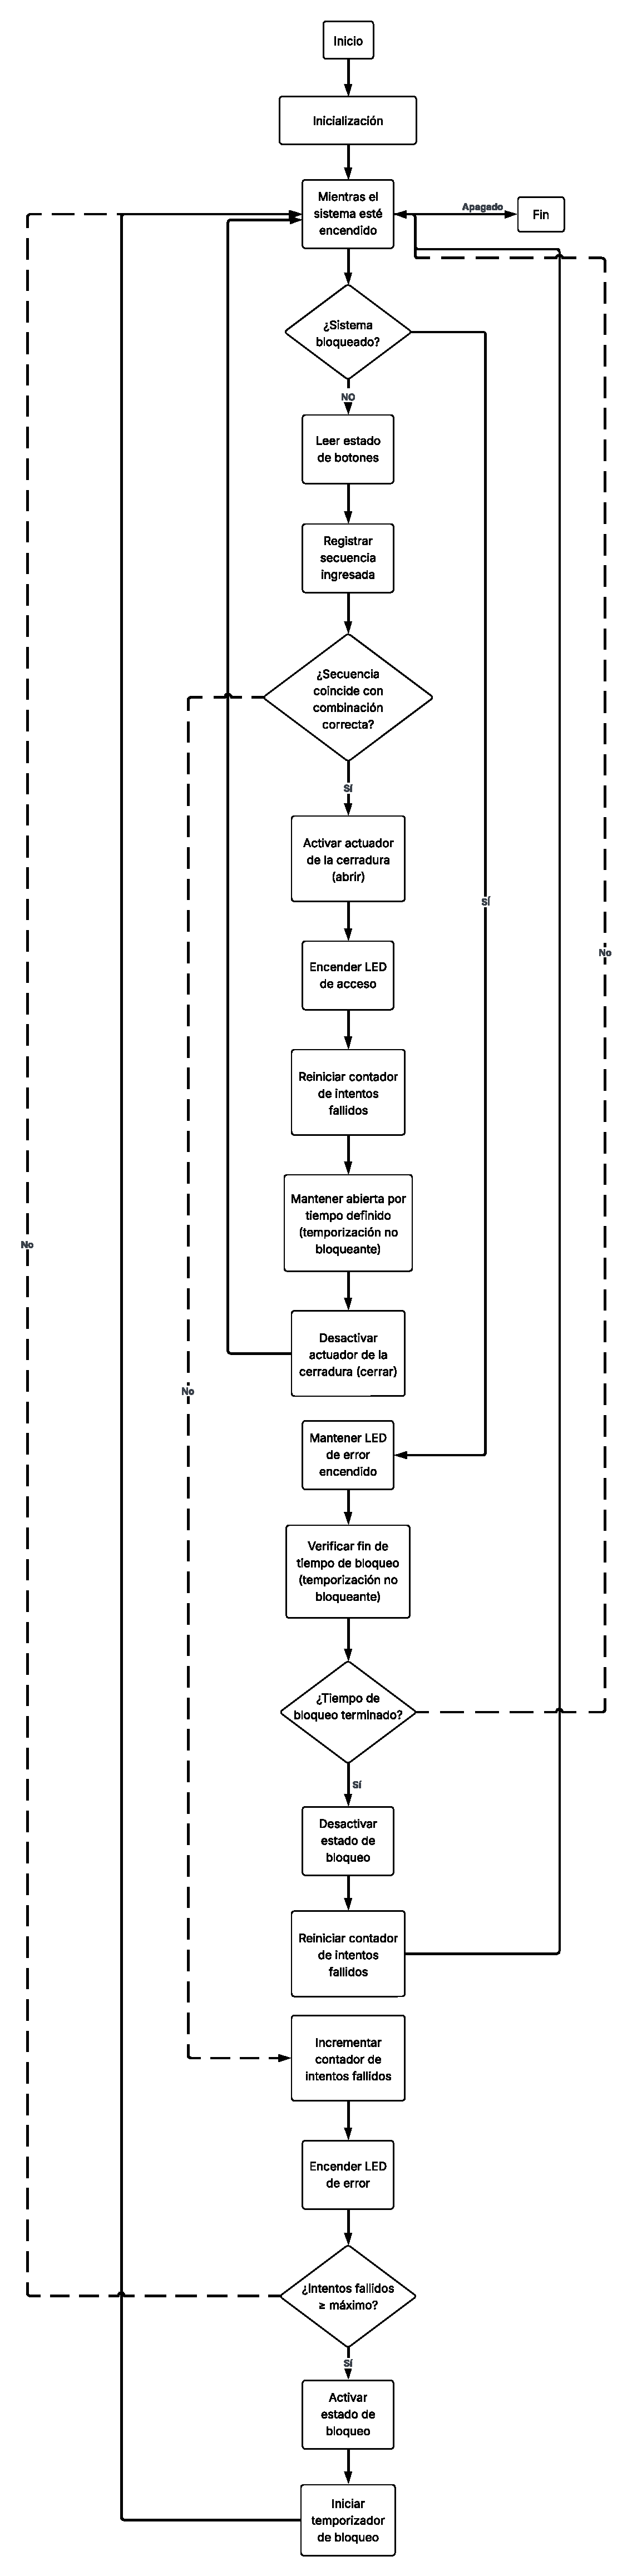
\includegraphics[width=0.3\textwidth]{images/Diagrama en blanco (3).pdf}
\caption{Flujograma reto 1} % Texto bajo la figura
  \label{Flujograma reto 1}          % Etiqueta para referenciar con \ref{fig:res_fig}
\end{figure}
\subsubsection{\textbf{Justificación técnica del microcontrolador seleccionado}}
\vspace{0,3cm}
\begin{itemize}
    \item \textbf{\textit{Número de pines requeridos:}}
    El sistema requiere tres pines de entrada digital para los botones utilizados en la combinación de acceso. Adicionalmente, se requieren dos pines de salida para los LED indicadores de estado (acceso autorizado y acceso denegado) y un pin de salida adicional para el control del actuador de la cerradura (servo motor o relé). En total se requieren aproximadamente seis pines GPIO. El ESP32 dispone de más de 30 pines de entrada/salida programables, por lo que cumple ampliamente con este requerimiento.

    \item \textbf{\textit{Capacidad de procesamiento:}}
    El microcontrolador cuenta con un procesador de doble núcleo basado en arquitectura Tensilica LX6 con frecuencia de operación de hasta 240 MHz, lo cual es suficiente para ejecutar la lógica de control del sistema, realizar la lectura de entradas digitales, gestionar temporizadores y generar señales PWM necesarias para el control de actuadores como servomotores. Su memoria RAM interna también permite implementar estructuras de datos para manejo de estados e intentos de autenticación.

    \item \textbf{\textit{Consumo energético:}}
    El ESP32 presenta un consumo aproximado entre 80 mA y 240 mA en modo activo dependiendo de la carga de procesamiento, y puede reducir su consumo a valores del orden de microamperios cuando se utilizan modos de bajo consumo como deep sleep. Esto resulta adecuado para sistemas de control que permanecen largos periodos en estado de espera.

    \item \textbf{Esquema de conexión:}
    Se encuentra en la imagen \ref{Diagrama de conexión reto 1}
\begin{figure}[H]
\centering
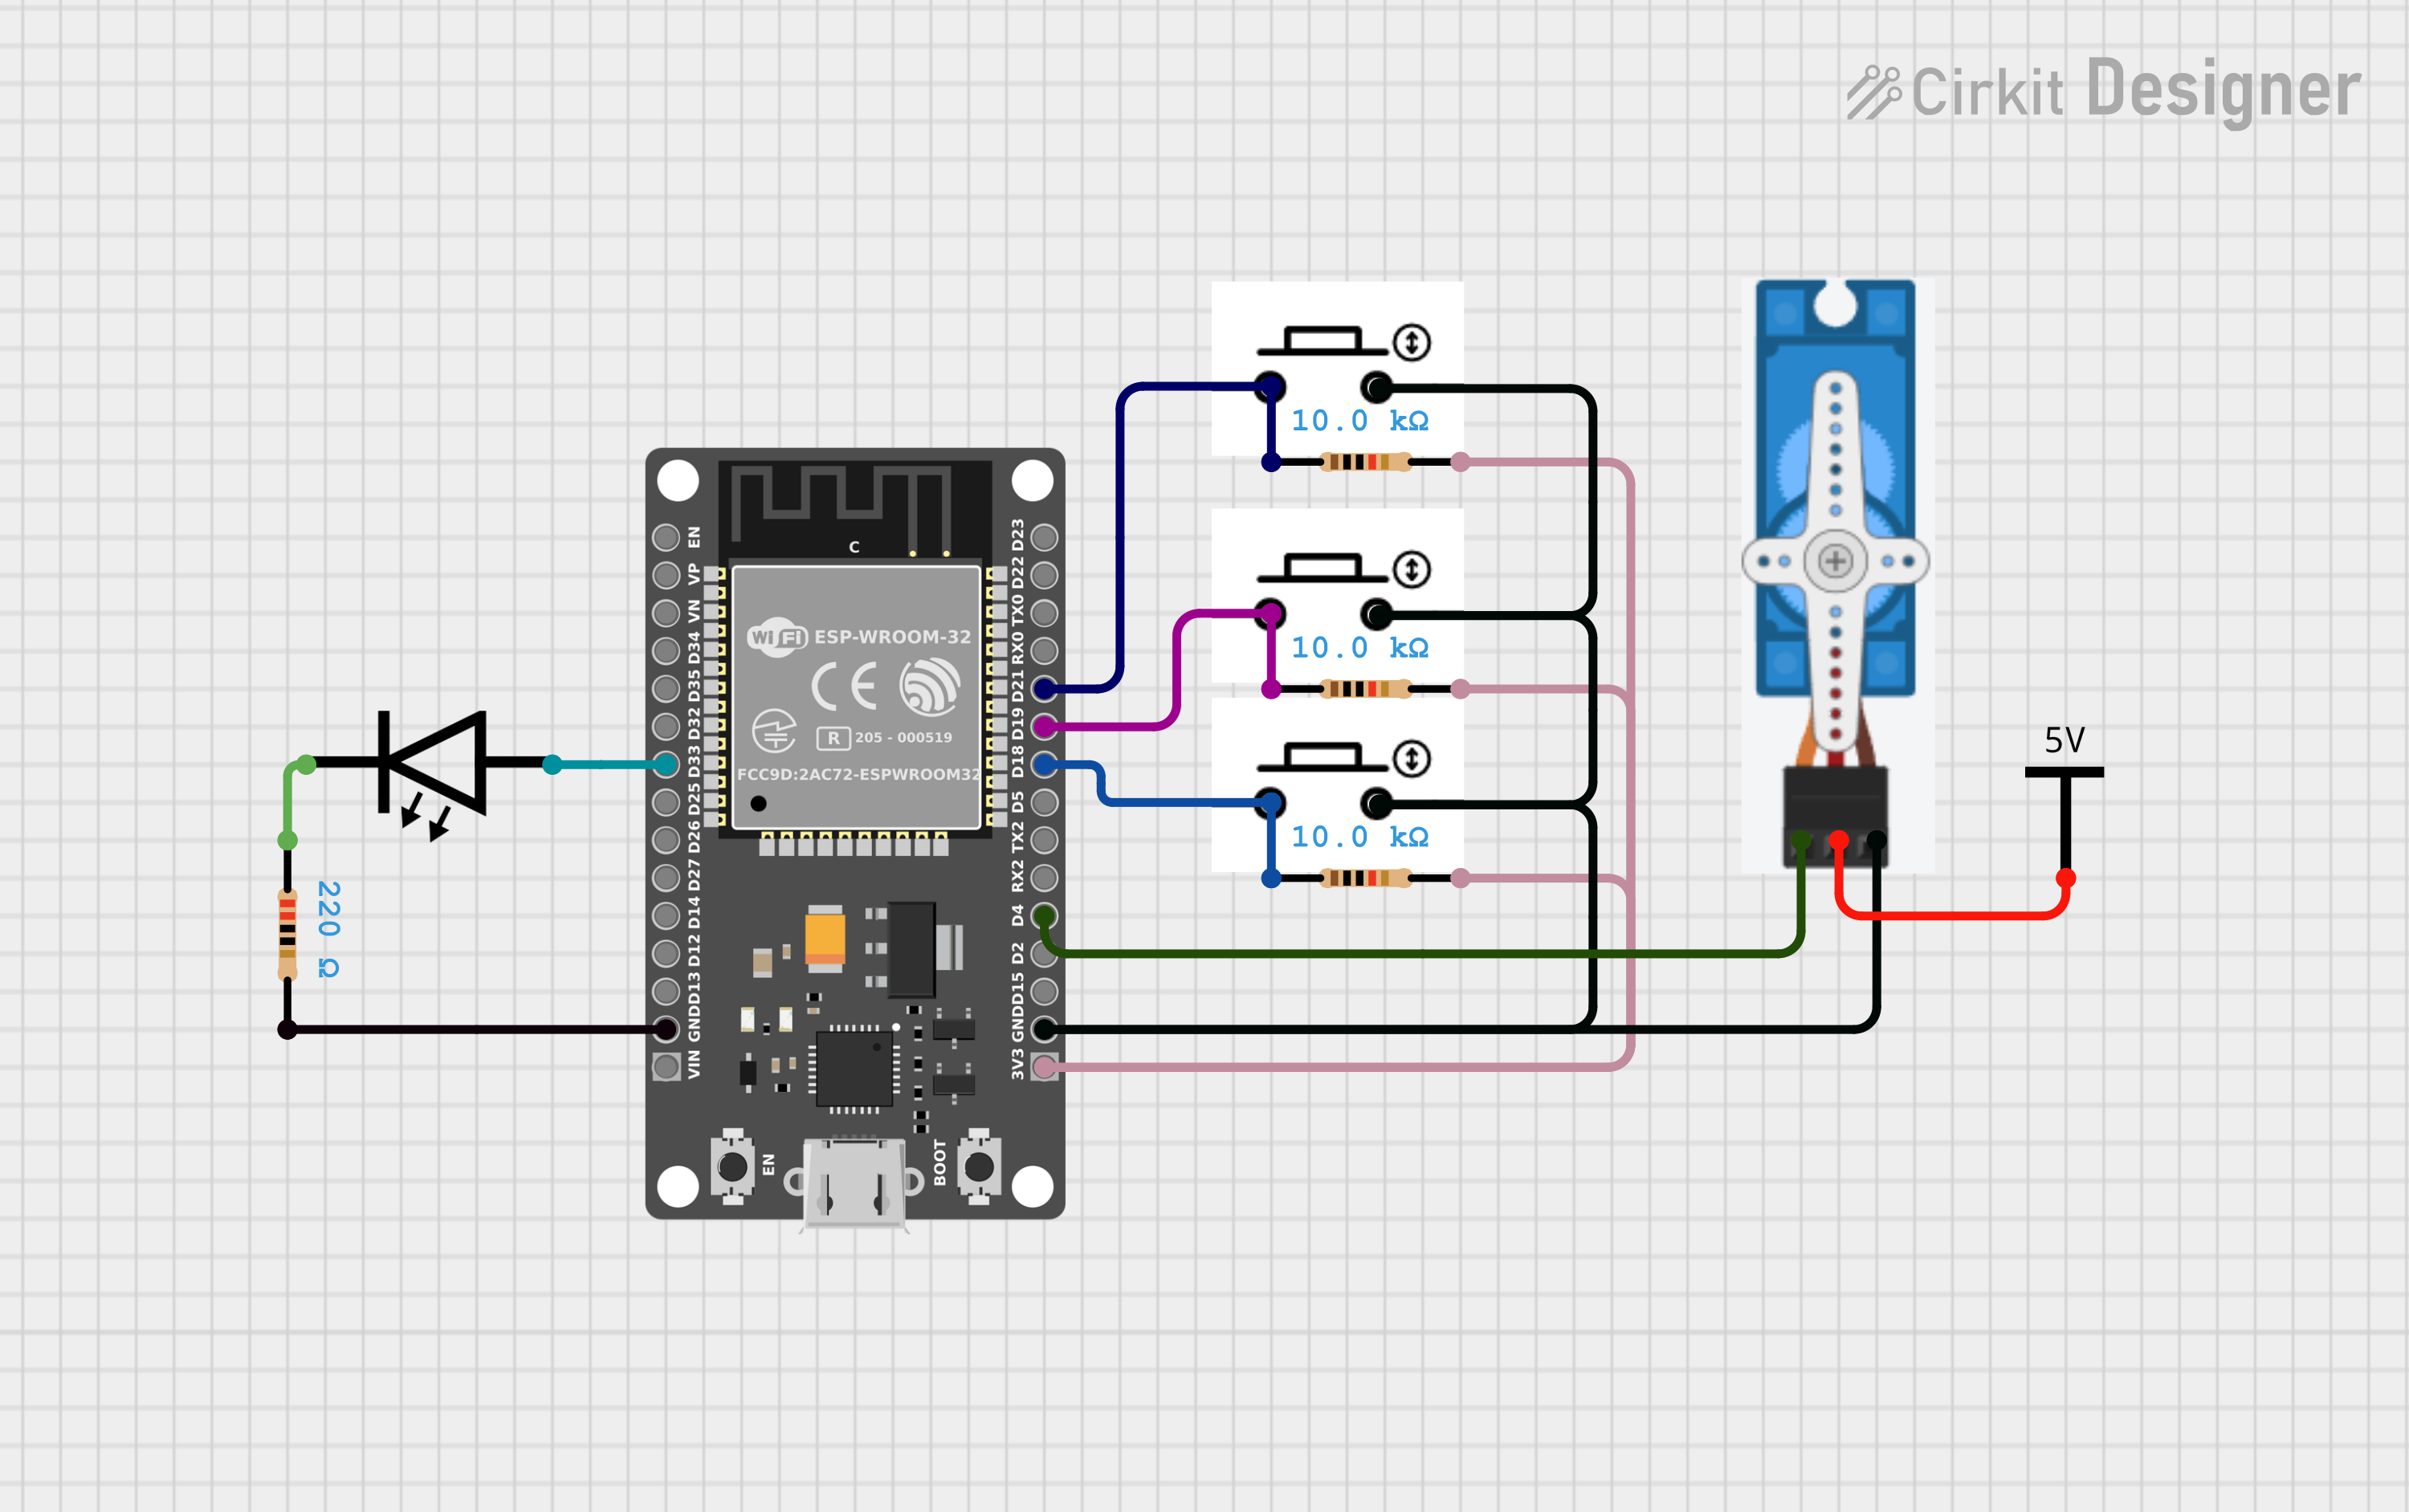
\includegraphics[width=0.4\textwidth]{images/Reto1.png}
\caption{Diagrama de conexión reto 1} % Texto bajo la figura
  \label{Diagrama de conexión reto 1}          % Etiqueta para referenciar con \ref{fig:res_fig}
\end{figure}

    \item \textbf{Componentes auxiliares}
    Para el correcto funcionamiento del sistema se requieren resistencias limitadoras de corriente para los LED (típicamente de 220 Ohm a 330 Ohm), resistencias de polarización para los botones (aproximadamente 10 kOhm), una fuente de alimentación estable para el microcontrolador y el actuador, y en caso de utilizar relé, un transistor driver con diodo de protección para evitar daños por voltajes inducidos. Estos componentes garantizan estabilidad eléctrica, protección de los dispositivos y operación confiable del sistema.
\end{itemize}
\subsubsection{\textbf{Código documentado}}
El código respectivo se encuentra en el anexo \ref{anexo:codigo1}

\subsection{\textbf{Reto 2}} % Sub-sección metodológica
Desarrollar un sistema que supervise una variable física y active alarmas según tres niveles de operación: normal, advertencia y crítico. Requisitos obligatorios:
\begin{itemize}
    \item Definición clara de umbrales
    \item Implementación de histéresis para evitar inestabilidad
    \item Indicadores visuales o sonoros
\end{itemize}
\vspace{0,3cm}
\subsubsection{\textbf{Análisis del problema}}
\begin{itemize}
    \item \textbf{\textit{Identificación de entradas y salidas:}} El sistema requiere una entrada correspondiente a la medición de una variable física que permita evaluar el estado del entorno supervisado. Para efectos de este diseño se selecciona la temperatura como variable de monitoreo, ya que constituye una de las variables más comunes en procesos industriales, sistemas electrónicos y aplicaciones de supervisión ambiental.

    La medición de la temperatura será realizada mediante un sensor de temperatura analógico, el cual entrega una señal proporcional a la magnitud física medida. Esta señal será adquirida por el microcontrolador a través de uno de sus canales de conversión analógico–digital (ADC), permitiendo así transformar la señal analógica en un valor digital interpretable por el sistema.

    En lo que corresponde a las salidas, el sistema contará con indicadores visuales y sonoros que permitirán identificar el estado operativo del sistema de monitoreo. Para ello se emplearán tres diodos LED que representarán los estados de operación normal, advertencia y condición crítica respectivamente. De manera adicional se incorporará una alarma sonora mediante un buzzer, el cual se activará únicamente cuando el sistema detecte que la variable monitoreada ha alcanzado el nivel crítico. 
\vspace{0,3cm}
    \item \textbf{\textit{Restricciones técnicas: }}
    \begin{itemize}
        \item El sensor de temperatura seleccionado entrega una señal analógica que debe ser interpretada por el microcontrolador \cite{LM35_datasheet}. Por lo tanto, el dispositivo de procesamiento debe contar con un convertidor analógico–digital con suficiente resolución para permitir una medición adecuada de la variable física.
        \item Los diodos LED empleados como indicadores visuales requieren la inclusión de resistencias limitadoras de corriente, ya que los pines GPIO del microcontrolador presentan límites de corriente que no deben ser superados para evitar daños en el dispositivo.
        \item En el caso del buzzer o alarma sonora, es necesario considerar que algunos dispositivos pueden requerir corrientes superiores a las que puede suministrar directamente un pin del microcontrolador\cite{buzzer_datasheet}. En estas condiciones puede ser necesario incorporar una etapa de conmutación basada en transistor, que permita manejar la carga sin comprometer la integridad del microcontrolador.
        \item Una restricción fundamental en este tipo de sistemas corresponde a la inestabilidad que puede presentarse cerca de los umbrales de decisión. Cuando la variable medida se encuentra próxima al valor límite entre dos estados, pequeñas fluctuaciones pueden provocar cambios continuos entre estados consecutivos. Para evitar este comportamiento se implementa un mecanismo de histéresis, el cual introduce un margen de diferencia entre los valores de activación y desactivación de cada estado \cite{temperature_hysteresis_cadence}.
    \end{itemize}
    \item 
    \textbf{\textit{Variables Involucradas:}}Variable que almacena el valor digital leído del convertidor analógico–digital correspondiente al sensor de temperatura. Variables que definen los umbrales del sistema para los estados normal, advertencia y crítico. Variable que indica el estado actual del sistema para activar los indicadores correspondientes. Variable que establece el margen de histéresis para evitar cambios repetitivos entre estados. Variables auxiliares para controlar el tiempo de muestreo y la frecuencia de lectura del sensor.
\end{itemize}

\subsubsection{\textbf{Flujograma del sistema}}
Se encuentra en la figura \ref{Flujograma reto 2}.
\begin{figure}
\centering
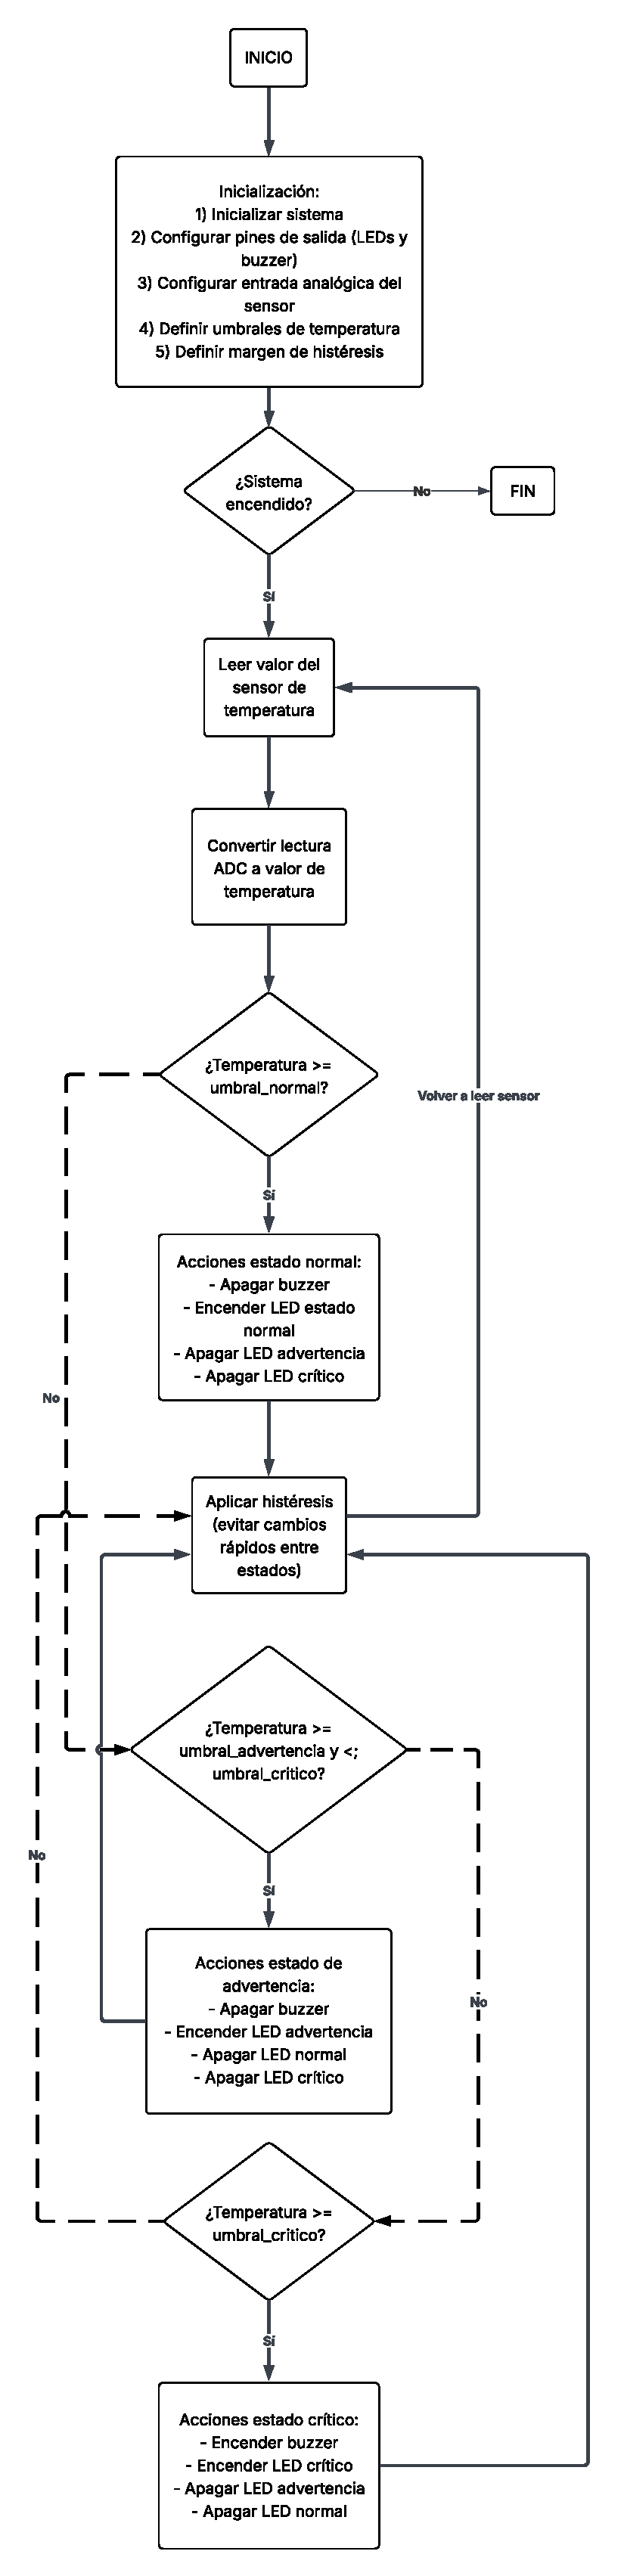
\includegraphics[width=0.3\textwidth]{images/Diagrama en blanco (1).pdf}
\caption{Flujograma reto 2} % Texto bajo la figura
  \label{Flujograma reto 2}          % Etiqueta para referenciar con \ref{fig:res_fig}
\end{figure}
\subsubsection{\textbf{Justificación técnica del microcontrolador seleccionado}}
\begin{itemize}
    \item \textbf{\textit{Número de pines requeridos.}}
    El sistema requiere al menos un pin de entrada analógica para la lectura del sensor que mide la variable física supervisada. Adicionalmente, se requieren tres pines de salida digital para los indicadores de estado correspondientes a los niveles de operación: normal, advertencia y crítico. También puede incorporarse un pin adicional para activar una alarma sonora mediante un buzzer. En total, el sistema requiere aproximadamente cinco pines de entrada/salida. El microcontrolador ESP32 dispone de múltiples pines GPIO y varios canales ADC de 12 bits \cite{espressif2021esp32}, lo que permite realizar la adquisición de la señal del sensor con suficiente resolución. 

    \item \textbf{\textit{Capacidad de procesamiento.}}
    El ESP32 cuenta con un procesador de doble núcleo con frecuencia de operación de hasta 240 MHz \cite{espressif2021esp32}, lo cual permite ejecutar el algoritmo de monitoreo en tiempo real, realizar la conversión analógica-digital de la señal del sensor y aplicar la lógica de comparación con los umbrales definidos. Además, su capacidad de procesamiento permite implementar histéresis en los niveles de alarma para evitar conmutaciones rápidas e inestables cuando la variable medida se encuentra cercana a los valores límite \cite{espressif2021esp32}.

    \item \textbf{\textit{Consumo energético.}}
    El dispositivo presenta un consumo aproximado entre 80 mA y 240 mA en modo activo, dependiendo de la carga de procesamiento y los periféricos utilizados. Asimismo, dispone de modos de bajo consumo que reducen significativamente la corriente cuando el sistema se encuentra en espera. Esto permite su utilización en sistemas de monitoreo continuo sin requerir un consumo energético elevado.

    \item \textbf{\textit{Esquema de conexión.}}
    Se encuentra en la imagen \ref{Diagrama de conexión reto 2}
\begin{figure}[H]
\centering
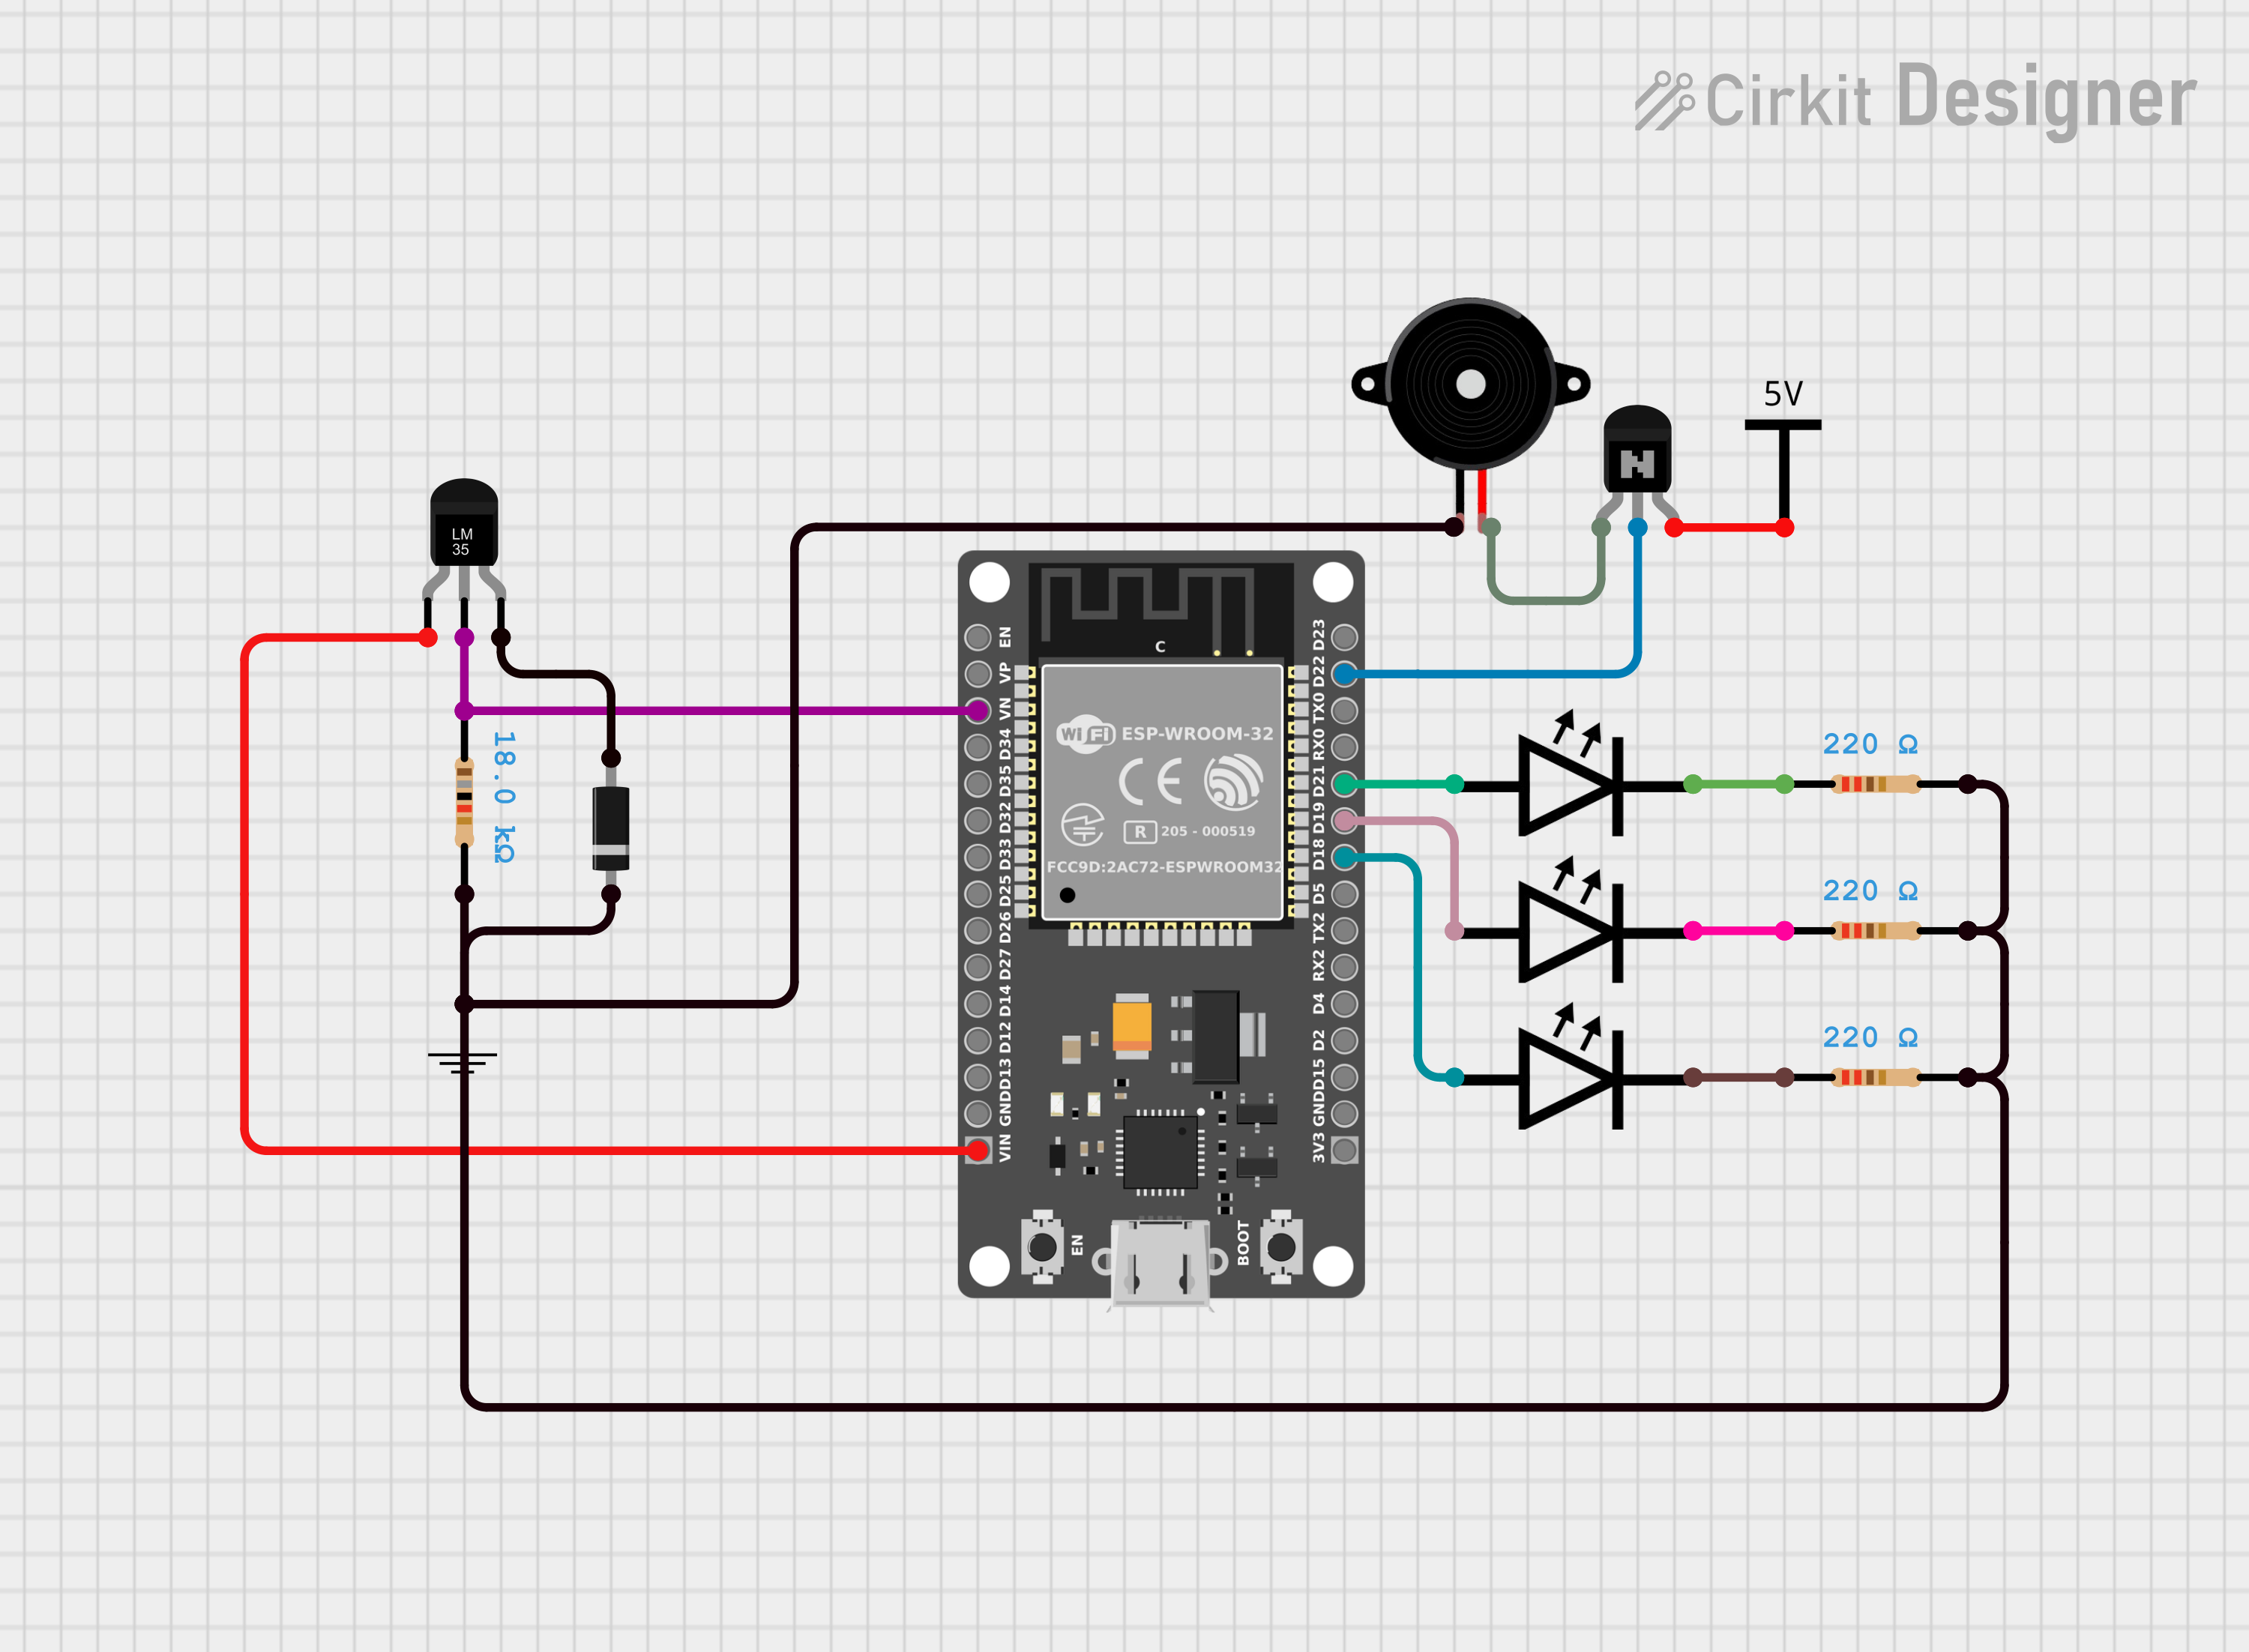
\includegraphics[width=0.4\textwidth]{images/Reto2.png}
\caption{Diagrama de conexión reto 2} % Texto bajo la figura
  \label{Diagrama de conexión reto 2}          % Etiqueta para referenciar con \ref{fig:res_fig}
\end{figure}

    \item \textbf{\textit{Componentes auxiliares}}
    El sistema requiere resistencias limitadoras de corriente para los LED indicadores (220 Ohm a 330 Ohm), resistencias de polarización en caso de utilizar sensores analógicos que lo requieran, y una fuente de alimentación estable para el microcontrolador y los dispositivos de salida. Si se emplea un buzzer activo o una alarma de mayor potencia, puede ser necesario utilizar un transistor driver para manejar la corriente requerida.
\end{itemize}

\subsubsection{\textbf{Código documentado}}
El código respectivo se encuentra en el anexo \ref{anexo:codigo2}

\subsection{\textbf{Reto 3}} % Sub-sección metodológica
Diseñar un sistema de riego automático para cultivo de tomate. El sistema debe: 
Monitorear la humedad del suelo,  
Activar riego cuando la humedad esté por debajo de un umbral, 
Detener el riego cuando se alcance nivel adecuado, 
Evitar inestabilidad mediante histéresis,  
Funcionar como sistema secuencial autónomo e  
Implemente temporización no bloqueante.


\subsubsection{\textbf{Análisis del problema}}
\begin{itemize}
    \item \textbf{\textit{Identificación de entradas y salidas:}}
    La entrada principal es un sensor de humedad del suelo conectado a una entrada analógica del microcontrolador. La salida corresponde al actuador de riego (bomba o válvula solenoide) controlado mediante un relé o transistor de potencia. Opcionalmente se puede incluir un LED indicador de estado del sistema.

    \item \textbf{\textit{Restricciones técnicas:}}
    \begin{itemize}
        \item El microcontrolador debe disponer de al menos una entrada analógica (ADC) para la lectura del sensor de humedad.

        \item Debe existir una salida digital capaz de controlar un relé o transistor para activar la bomba o válvula de riego.

        \item El sistema debe operar con niveles de voltaje compatibles (3.3 V o 5 V) entre microcontrolador, sensor y etapa de potencia. \cite{espressif2021esp32}

        \item El control del riego debe implementar histéresis mediante dos umbrales de humedad para evitar conmutaciones rápidas.

        \item El software debe emplear temporización no bloqueante (por ejemplo mediante contadores de tiempo) para permitir lecturas periódicas del sensor.

    \end{itemize}

    \item \textbf{\textit{Variables involucradas:}}
    Las variables principales son el valor de humedad del suelo medido por el sensor, el umbral inferior de activación del riego, el umbral superior de desactivación, el estado del sistema (riego activo o inactivo) y las variables de temporización utilizadas para el muestreo periódico del sensor.
\end{itemize}

\subsubsection{\textbf{Flujograma del sistema} }
Se encuentra en la figura \ref{Flujograma reto 3}
\begin{figure}
\centering
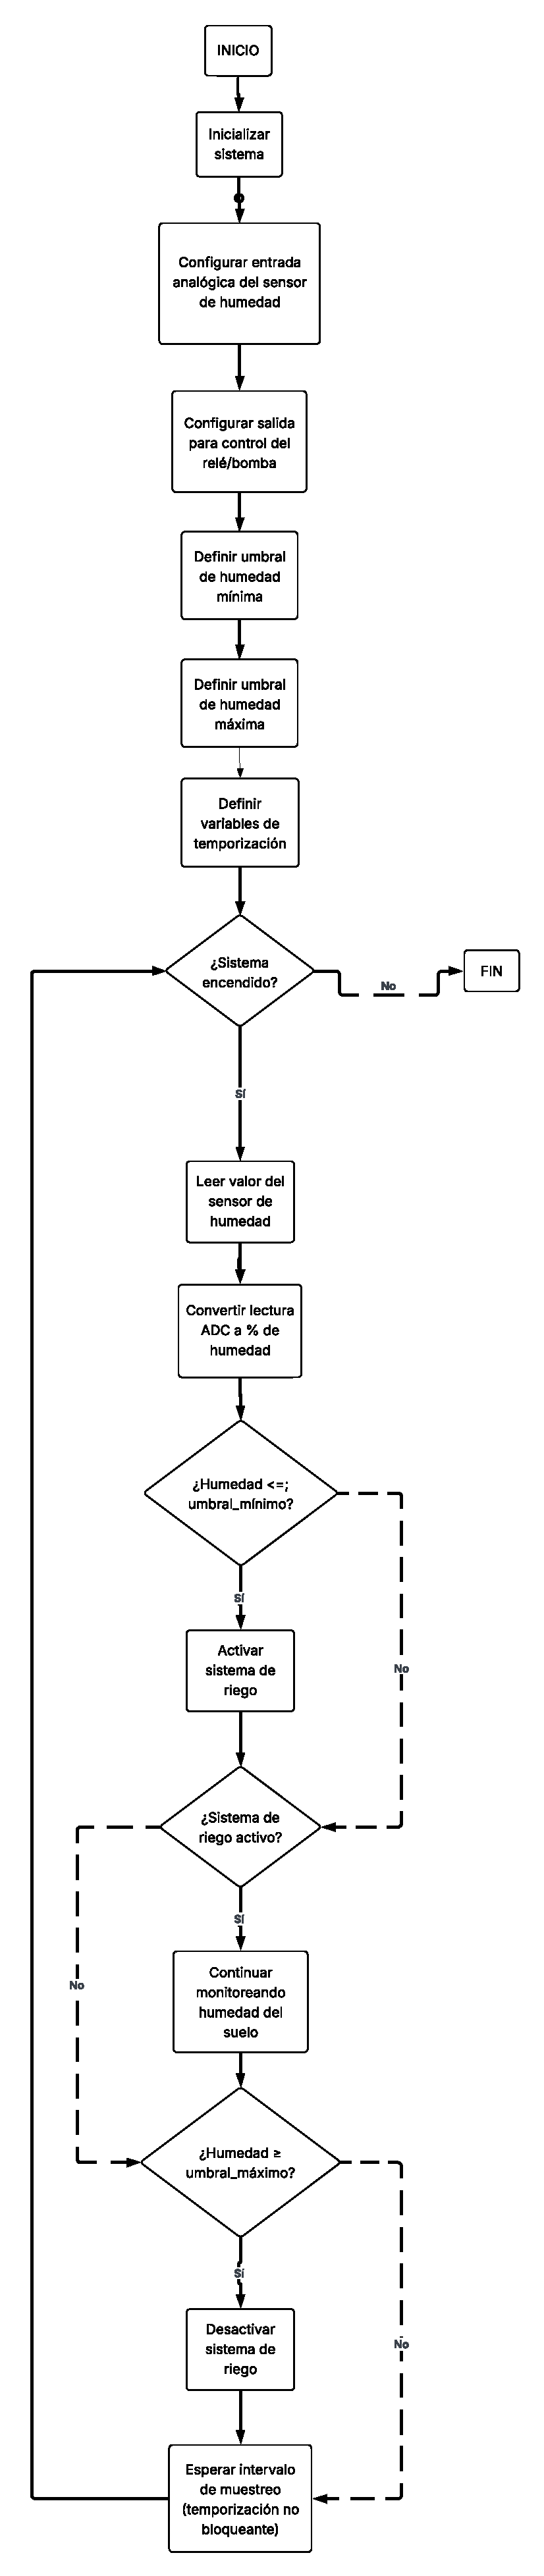
\includegraphics[width=0.25\textwidth]{images/Diagrama en blanco (2).pdf}
\caption{Flujograma reto 3} % Texto bajo la figura
  \label{Flujograma reto 3}          % Etiqueta para referenciar con \ref{fig:res_fig}
\end{figure}
\subsubsection{\textbf{Justificación técnica del microcontrolador seleccionado}}
\begin{itemize}
    \item \textbf{\textit{Número de pines requeridos:}}
    El sistema requiere 1 entrada analógica para el sensor de humedad del suelo y 1 salida digital para controlar el relé o transistor que activa la bomba de riego. Opcionalmente se puede utilizar 1 salida digital adicional para un LED indicador. El ESP32 dispone de más de 30 pines GPIO, incluyendo múltiples entradas ADC, por lo que satisface ampliamente los requerimientos del sistema. 

    \item \textbf{\textit{Capacidad de procesamiento:}}
    El ESP32 integra un procesador dual-core de hasta 240 MHz \cite{espressif2021esp32}, suficiente para ejecutar el algoritmo de control secuencial, realizar lecturas periódicas del sensor mediante ADC, aplicar histéresis entre umbrales de humedad y gestionar temporización no bloqueante para el monitoreo continuo del sistema.

    \item \textbf{\textit{Consumo energético:}}
    El microcontrolador opera a 3.3 V y presenta un consumo aproximado de 80–240 mA en operación \cite{espressif2021esp32}, con modos de bajo consumo disponibles. Esto permite su integración en sistemas agrícolas automatizados con alimentación estable o mediante fuentes reguladas.

    \item \textbf{\textit{Esquema de conexión (diagrama eléctrico o esquemático):}}
    Se encuentra en la imagen \ref{Diagrama de conexión reto 3}
\begin{figure}[H]
\centering
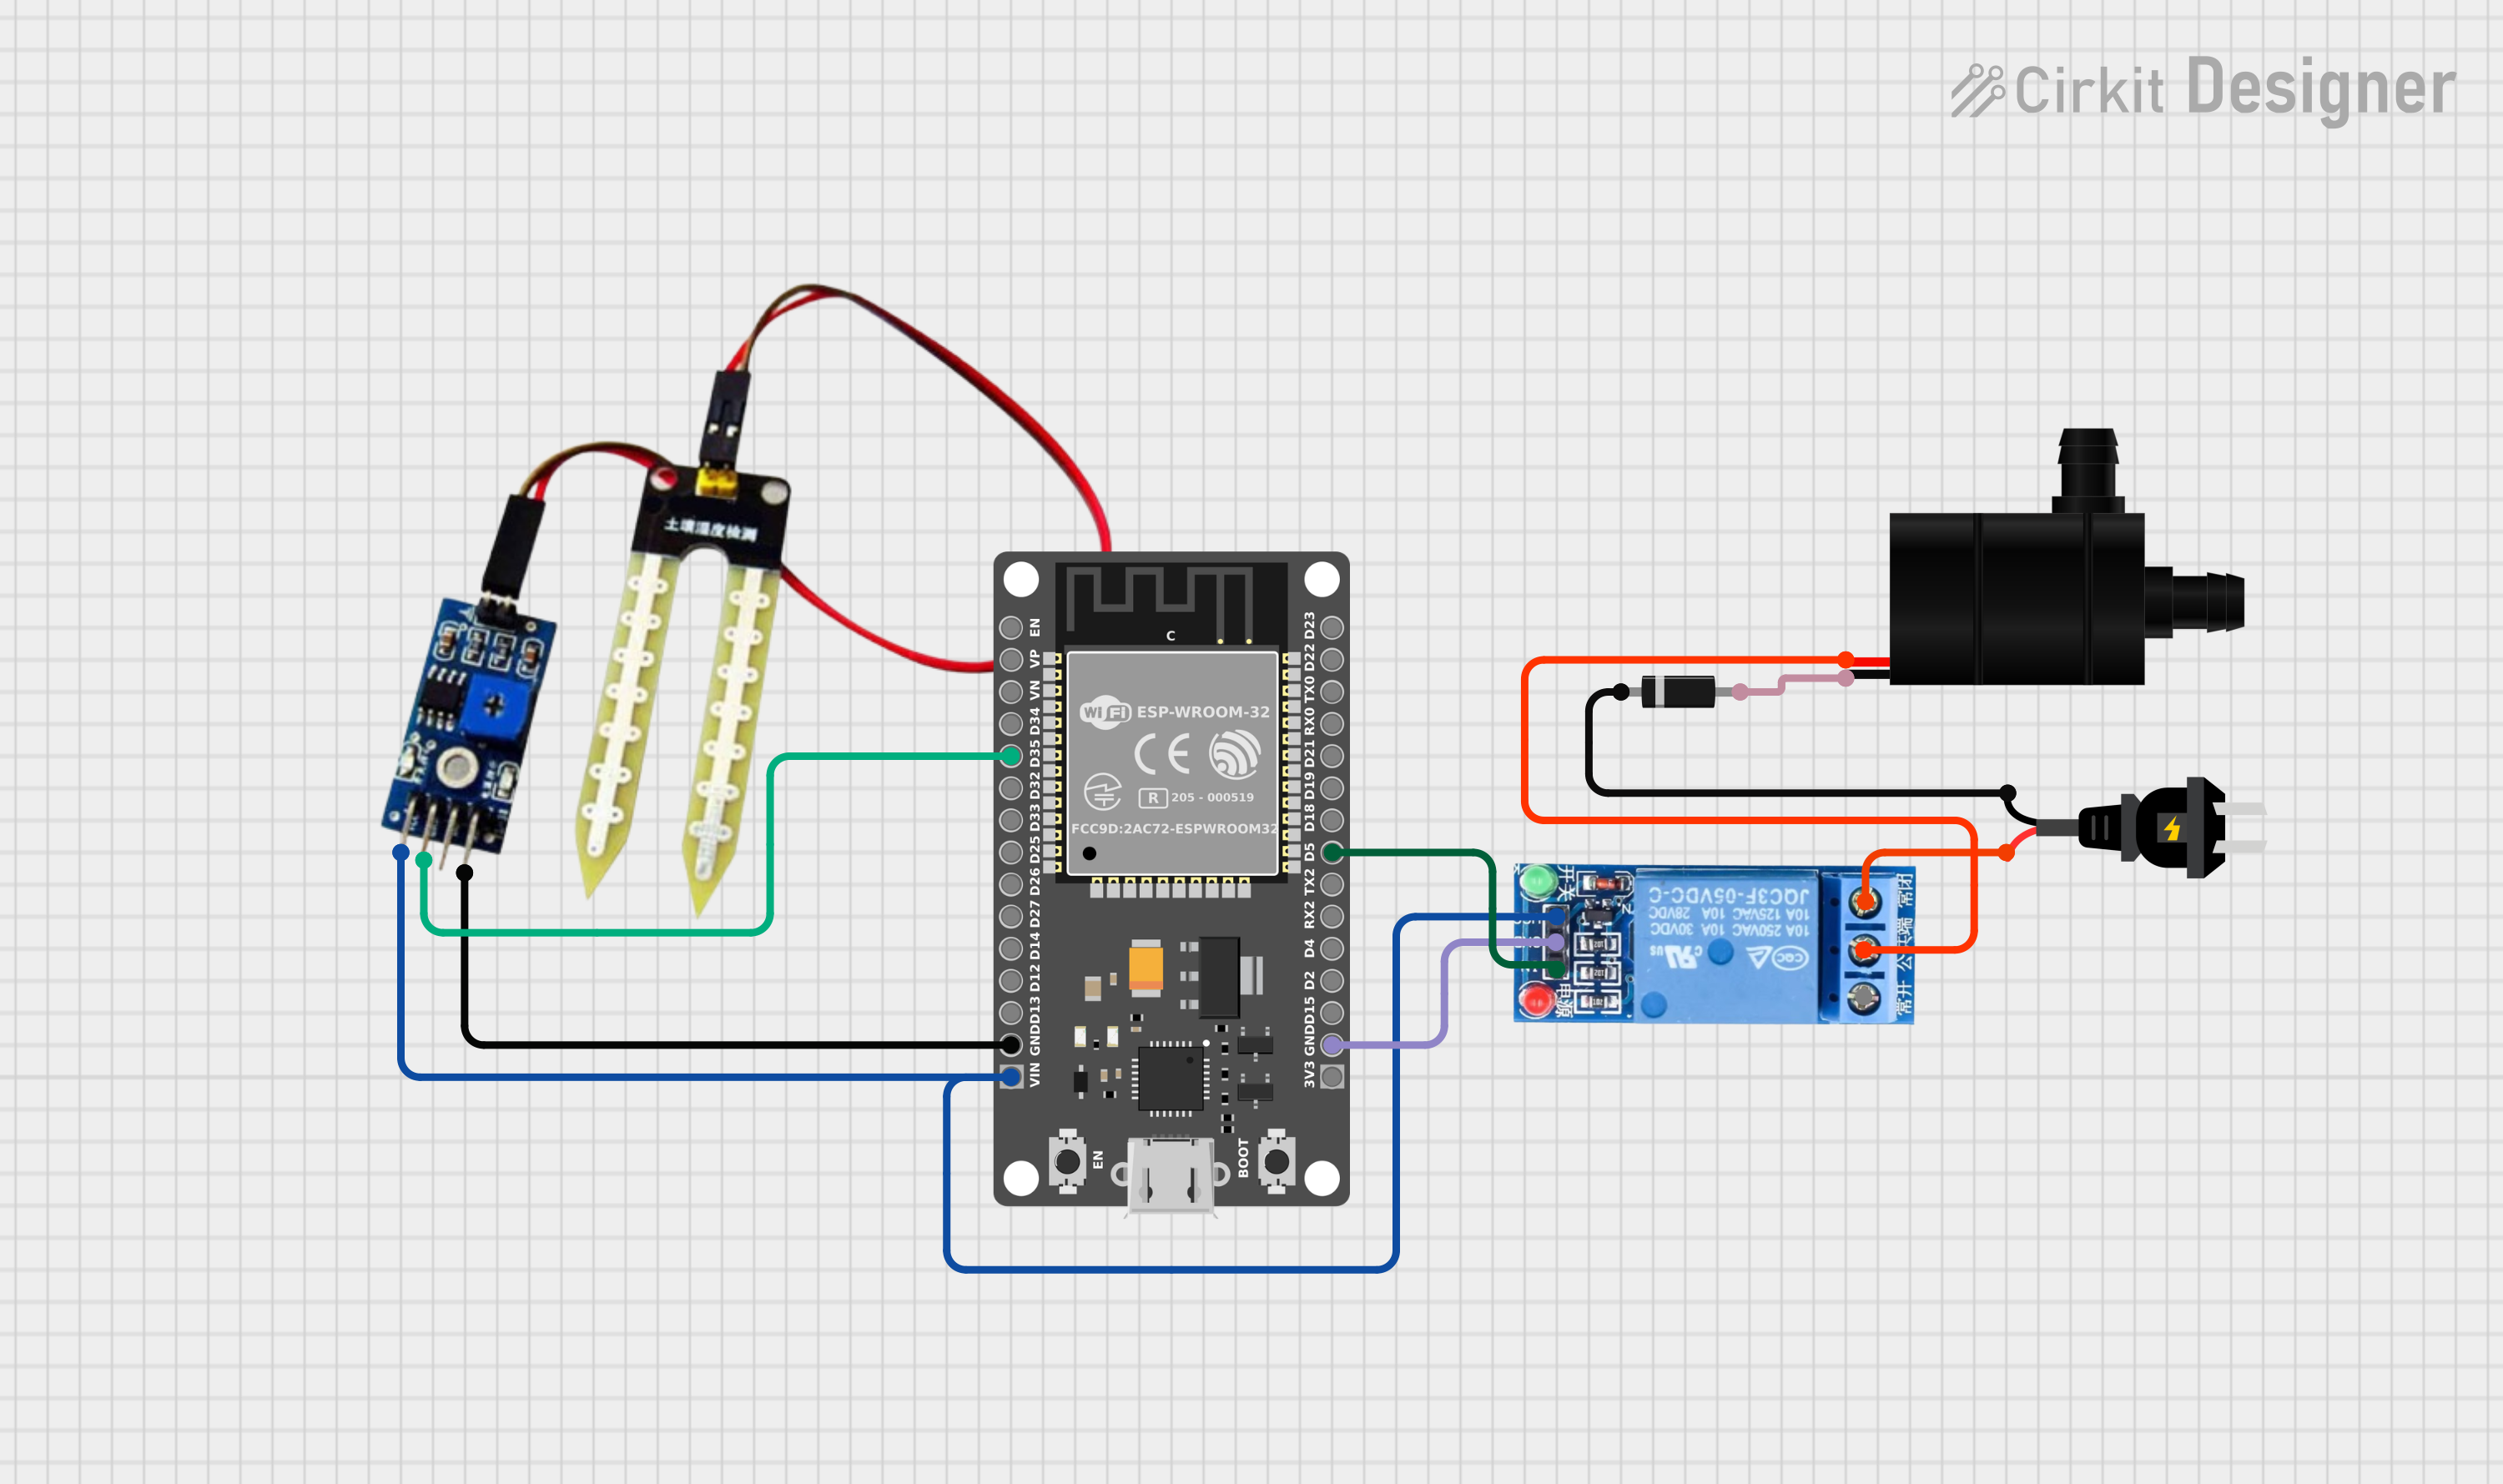
\includegraphics[width=0.4\textwidth]{images/Reto3.png}
\caption{Diagrama de conexión reto 3} % Texto bajo la figura
  \label{Diagrama de conexión reto 3}          % Etiqueta para referenciar con \ref{fig:res_fig}
\end{figure}

    \item\textbf{\textit{Componentes auxiliares}} El sistema requiere un sensor de humedad del suelo, un módulo relé o MOSFET de potencia, resistencias de polarización para el control del transistor, diodo de protección, una bomba de agua o válvula solenoide para el riego y opcionalmente LEDs indicadores para mostrar el estado del sistema.
\end{itemize}
\subsubsection{\textbf{Código documentado}}
El código respectivo se encuentra en el anexo \ref{anexo:codigo3}


